%!TEX root = ../../report.tex
\section{Costmap for Path Planning}
\label{sec:cost_interpretation_path_planning}
The path planning uses the costmap to determine the path with the lowest cost while avoiding lethal obstacles. 
The path planner uses lethal as well as non-lethal costs to accomplish this. 
Therefore, the dynamic obstacle should be represented to help guide the path planning away from obstacles that might obstruct the path and possibly cause a re-planning. 
Because path planning is most likely handled without observing most of the path the cost of cells have to be predicted. 
The Markov model used in the Dynamic learner is well suited to estimate the probabilities for being in the free or occupied state. 
Given the time since the last observation it is possible to calculate the number of steps the Markov chain must go through to project the state to the current time.
The predictions are performed from the estimated occupancy probability, which is updated with new measurements.

\subsection{Occupancy Estimation Update}
A simple update of the estimated occupancy probability would be to override it with the latest observation.  
A problem with this is uncertainty in observations. 
If an observation is very uncertain ($\approx0.5$), it carries very little information and therefore not very suitable to be used in the forward projection. 
As it is not desirable to use such uncertain values as basis for the forward projection, an update and predict scheme is used.
Each time a new value is received the current occupancy probability estimate, \(\hat{p}_{occ}(t)\), is updated as shown in equation \ref{eq:cost_update}.
%
\begin{equation}
\label{eq:cost_update}
\hat{p}_{occ}(t) = \hat{p}_{occ}(t-1) +  2  \left\| p_{occ} - 0.5 \right\| \cdot \left[p_{occ} - \hat{p}_{occ}(t-1) \right]  
\end{equation}
%
The correction value is the difference between the new measurement and the previous estimate.
This is weighted according to the certainty in the new observation.  
Figure \ref{fig:cost_update} shows an example of the update method for the \(\hat{p}_{occ}\). 
\begin{figure}[htbp]
	\centering
	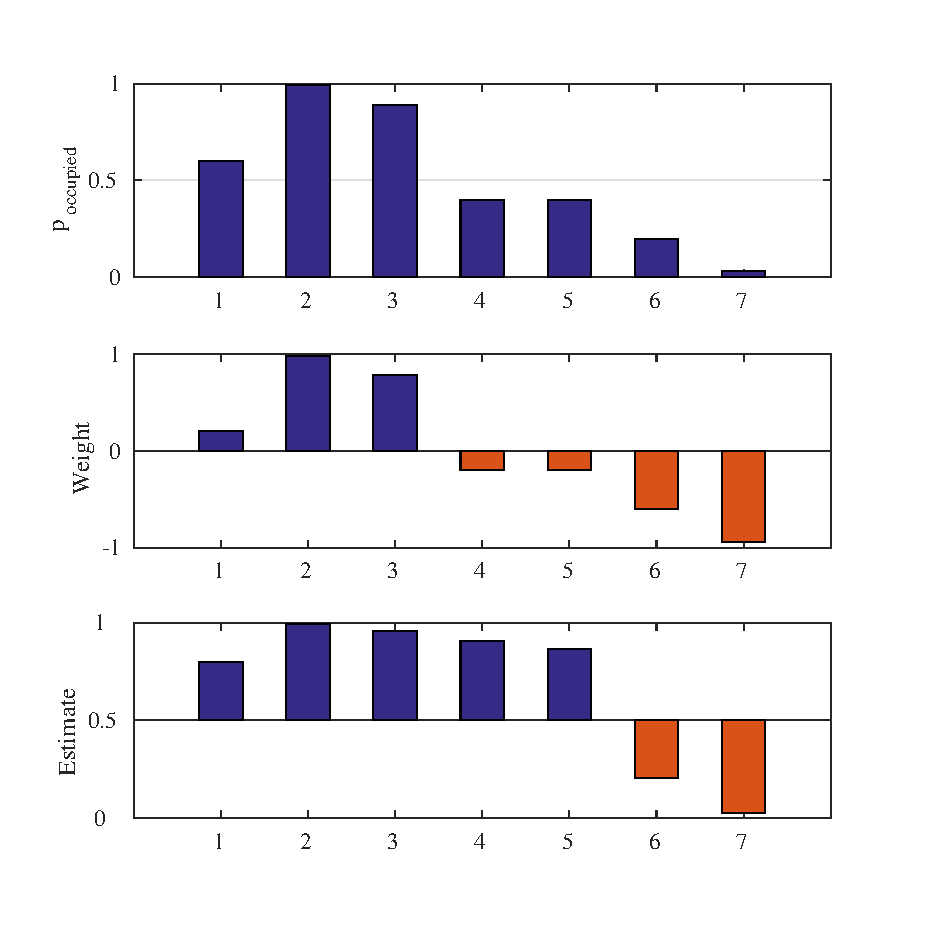
\includegraphics[width=1\linewidth]{chapters/cost_interpretation/figures/update}
	\caption{Update of the estimated occupancy. Sign in weight indicates free or occupied, positive is occupied. }
	\label{fig:cost_update}
\end{figure}
\todo{axis x -> t}
It is seen in figure \ref{fig:cost_update} that the uncertain free values does not cause a great shift in the estimated occupancy value. When the free observations become increasingly certain a significant change is observed. 

\subsection{Occupancy Prediction}
The predict steps are performed when a new map is to be generated. At this time all cells are projected forward from their last observed time to the current time. This is done by using the estimated occupancy as the initial distribution and then projecting forward a number of steps according to the time difference between last observation and the current time.
Equation \ref{eq:markov_project} shows the $n$ step projection of the estimated occupancy probability.
\begin{equation}
\label{eq:markov_project}
\begin{bmatrix}
1-p_{proj} & p_{proj}
\end{bmatrix}
=
\begin{bmatrix}
1-\hat{p}_{occ} & \hat{p}_{occ}
\end{bmatrix}
\cdot
\begin{bmatrix}
1 - \hat{\lambda}_{entry} & \hat{\lambda}_{entry}\\ 
\hat{\lambda}_{exit} & 1- \hat{\lambda}_{exit}
\end{bmatrix}^n
\end{equation}
If the number of steps to project is larger than five, then the estimate is not used. Instead the stationary distribution in  equation \ref{eq:long_term} determines the final occupancy probability \cite{Meyer-Delius2012}.
\begin{equation}
	\label{eq:long_term}
	p_{stationary} = \frac{1}{\lambda_{entry} + \lambda_{exit}} \cdot \lambda_{entry}
\end{equation}

Figure \ref{fig:cost_predict} shows the projection of a cell with the Markov parameters \(p_{exit} = 0.13 \) and \(p_{entry} = 0.52 \). 
The initial probability estimate is the last estimate from figure \ref{fig:cost_update}. 
It is clear that in this case, it does not take many forward projection until it converges close to the long term. 

\begin{figure}[htbp]
	\centering
	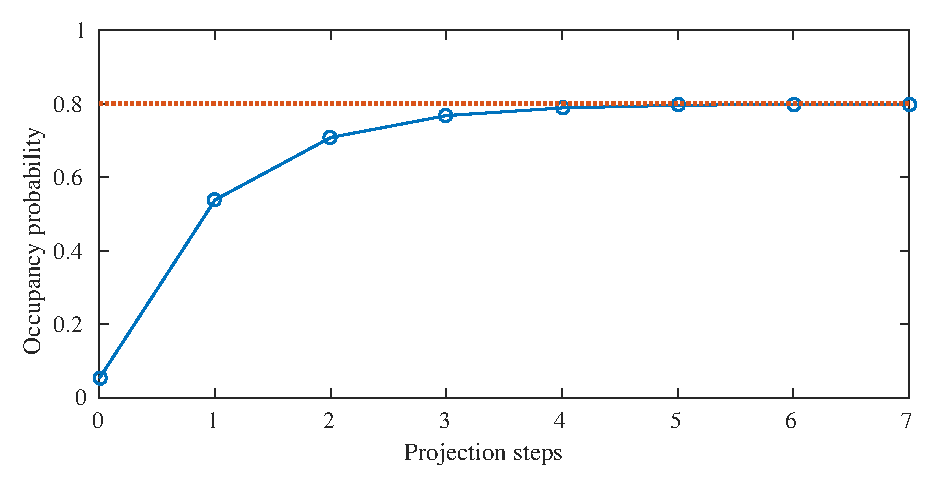
\includegraphics[width=1\linewidth]{chapters/cost_interpretation/figures/projection}
	\caption{Prediction of occupancy. Markov parameters: \(\lambda_{entry} = 0.52\), \(\lambda_{exit} = 0.13\)}
	\label{fig:cost_predict}
\end{figure}

\subsection{Converting Probability to Cost}
The cost assigned to the costmap is controlled by the function $\phi(p)$. Its input is the occupancy probabilities calculated by the prediction methods.
The function scales the probability into the cost range assigned to dynamic obstacles.
The cost $\kappa$ depends on $n$ as shown in equation \ref{eq:cost_conversion}.
The nature of the function $\phi$ depends on the path planner and demands for the path. 

\begin{equation}
\label{eq:cost_conversion}
\kappa = 
\begin{cases}
\phi(p_{proj}), & \text{if } n \le 5
\\
\phi(p_{stationary}), & \text{otherwise}
\end{cases}
\end{equation}